\documentclass{beamer}
\usepackage[utf8]{inputenc}
\usetheme{Madrid}
\usecolortheme{default}
\usepackage{amsmath,amssymb,amsfonts,amsthm}
\usepackage{txfonts}
\usepackage{tkz-euclide}
\usepackage{listings}
\usepackage{adjustbox}
\usepackage{array}
\usepackage{tabularx}
\usepackage{gvv}
\usepackage{lmodern}
\usepackage{circuitikz}
\usepackage{tikz}
\usepackage{graphicx}
\usepackage{etoolbox}
\setbeamertemplate{page number in head/foot}[totalframenumber]

\usepackage{tcolorbox}
\tcbuselibrary{minted,breakable,xparse,skins}



\definecolor{bg}{gray}{0.95}
\DeclareTCBListing{mintedbox}{O{}m!O{}}{%
  breakable=true,
  listing engine=minted,
  listing only,
  minted language=#2,
  minted style=default,
  minted options={%
    linenos,
    gobble=0,
    breaklines=true,
    breakafter=,,
    fontsize=\small,
    numbersep=8pt,
    #1},
  boxsep=0pt,
  left skip=0pt,
  right skip=0pt,
  left=25pt,
  right=0pt,
  top=3pt,
  bottom=3pt,
  arc=5pt,
  leftrule=0pt,
  rightrule=0pt,
  bottomrule=2pt,
  toprule=2pt,
  colback=bg,
  colframe=orange!70,
  enhanced,
  overlay={%
    \begin{tcbclipinterior}
    \fill[orange!20!white] (frame.south west) rectangle ([xshift=20pt]frame.north west);
    \end{tcbclipinterior}},
  #3,
}
\lstset{
    language=C,
    basicstyle=\ttfamily\small,
    keywordstyle=\color{blue},
    stringstyle=\color{orange},
    commentstyle=\color{green!60!black},
    numbers=left,
    numberstyle=\tiny\color{gray},
    breaklines=true,
    showstringspaces=false,
}
%------------------------------------------------------------
%This block of code defines the information to appear in the
%Title page
\title %optional
{1.2.24}

%\subtitle{A short story}

\author % (optional)
{Varun-ai25btech11016}



\begin{document}


\frame{\titlepage}
\begin{frame}{Question}
Rain is falling vertically with a speed of 35 m/s. Wind starts blowing after some time with a speed of 12 m/s in the east to west direction. In which direction should a boy waiting at a bus stop hold his umbrella?\\

\end{frame}



\begin{frame}{Theoretical Solution }

 Let,


$\vec{v}_{r/w}$ be the velocity of rain relative to the wind (downward), 
$$\vec{v}_{r/w}=\begin{myvec}{0\\-35}\end{myvec}$$.

$\vec{v}_{w}$ be the velocity of wind relative to ground 

$$\vec{v}_{w}=\begin{myvec}{-12\\0}\end{myvec}$$.

$\vec{v}_{r}$ be the velocity of rain relative to ground 
Take $+x$ to the east and $+y$ upward.


\textbf{Resultant rain velocity (relative to ground).}
\begin{align}
    \vec{v}_{r} &= \vec{v}_{w} + \vec{v}_{r/w}
\end{align}


Let $\theta$ be the angle between $\vec{v}_{r}$ and the downward vertical unit vector $$\hat{u}_{\downarrow}=\begin{myvec}{0\\-1}\end{myvec}$$.

\end{frame}
\begin{frame}{Theoretical Solution}


Using the dot product,
\begin{align}
    \cos\theta &= \frac{\vec{v}_{r}\cdot \hat{u}_{\downarrow}}{\|\vec{v}_{r}\|} \\
    \cos\theta &= \frac{v_{r/w}}{\sqrt{v_{r/w}^2 + v_w^2}}
\end{align}
\text{Equation 3 is obtained by substituting Equation 1 in Equation 2 }

\end{frame}
\begin{frame}{Theoretical Solution}
\textbf{Substitute given values.}

For this problem, the speed of rain w.r.t wind is $v_{r/w}=35\ \text{m/s}$ 

the wind speed is $v_w=12\ \text{m/s}$ (east to west).
\begin{align}
    \cos\theta &= \frac{35}{\sqrt{35^2 + 12^2}} \\
    \cos\theta &= \frac{35}{37} \\ 
        \theta &= \cos^{-1}\!\left(\frac{35}{37}\right)
\end{align}

\end{frame}
\begin{frame}{Conclusion} 
Rain falls at an angle of 
$\theta=\cos^{-1}\!\left(\frac{35}{37}\right)$ west of vertical downward

The rain’s velocity component is toward the west and downward, so the umbrella must be kept in the opposite direction:

Hence,
\begin{align}
 \text{Umbrella direction should be at an angle} \cos^{-1}\!\left(\frac{35}{37}\right)\ \text{east of vertical upward.}
\end{align}

\end{frame}


\begin{frame}[fragile]
    \frametitle{C Code }
\begin{lstlisting}
#include <math.h>
#include<stdio.h>
// Function to compute umbrella angle (in radians)
// vrw = velocity of rain relative to wind (2D vector)
// vw  = velocity of wind relative to ground (2D vector)
double umbrella_angle(double vrw[2], double vw[2]) {
    // Step 1: Resultant rain velocity relative to ground
    double vr[2];
    vr[0] = vw[0] + vrw[0];
    vr[1] = vw[1] + vrw[1];

    // Step 2: Downward unit vector
    double u_{down}[2] = {0.0, -1.0};
 \end{lstlisting}
\end{frame}
\begin{frame}[fragile]
    \frametitle{C Code }
    
\begin{lstlisting}
    // Step 3: Dot product
    double dot = vr[0]*u_down[0] + vr[1]*u_down[1];

    // Step 4: Norm of vr
    double norm_vr = sqrt(vr[0]*vr[0] + vr[1]*vr[1]);

    // Step 5: Angle from vertical (acos of normalized dot product)
    return acos(dot / norm_vr);   // radians

 \end{lstlisting}
\end{frame}


\begin{frame}[fragile]
    \frametitle{Python+C code}
    \begin{lstlisting}

import ctypes
import numpy as np
import matplotlib.pyplot as plt
import math
import os

# ---- load the shared library (must be in same folder) ----
lib_path = "./umbrella.so"


lib = ctypes.CDLL(lib_path)
lib.umbrella_angle.argtypes = [ctypes.c_double * 2, ctypes.c_double * 2]
lib.umbrella_angle.restype = ctypes.c_double
 \end{lstlisting}
\end{frame}
\begin{frame}[fragile]
    \frametitle{Python+C code}
    \begin{lstlisting}


vrw_np = np.array([0.0, -35.0])   # rain relative to wind (x east, y up)
vw_np  = np.array([-12.0, 0.0])   # wind (east->west is -12)

# prepare ctypes arrays and call C function
vrw_ct = (ctypes.c_double * 2)(*vrw_np)
vw_ct  = (ctypes.c_double * 2)(*vw_np)

theta = lib.umbrella_angle(vrw_ct, vw_ct)   # radians returned from C
theta_deg = math.degrees(theta)

printf("Angle from vertical (radians): {theta:.6f}")
printf("Angle from vertical (degrees): {theta_deg:.3f}")
\end{lstlisting}
\end{frame}
\begin{frame}[fragile]
    \frametitle{Python+C code}
    \begin{lstlisting}

# ---- prepare plotting data ----
v_r = vrw_np + vw_np                 # resultant rain velocity (ground frame)
umbrella_dir = -v_r                  # umbrella points opposite to rain motion
# scale umbrella arrow so it's visible on the plot (preserve direction)
if np.linalg.norm(umbrella_dir) > 0:
    umbrella_vis = umbrella_dir / np.linalg.norm(umbrella_dir) * 20.0
else:
    umbrella_vis = np.array([0.0, 0.0])

# ---- plotting ----
fig, ax = plt.subplots(figsize=(7,7))
\end{lstlisting}
\end{frame}
\begin{frame}[fragile]
    \frametitle{Python+C code}
    \begin{lstlisting}



ax.quiver(0, 0, vrw_np[0], vrw_np[1], angles='xy', scale_units='xy', scale=1,
          color='tab:blue', width=0.006, label=r'$\vec v_{r/w}=(0,-35)$')
ax.quiver(0, 0, vw_np[0], vw_np[1], angles='xy', scale_units='xy', scale=1,
          color='tab:green', width=0.006, label=r'$\vec v_w=(-12,0)$')
ax.quiver(0, 0, v_r[0], v_r[1], angles='xy', scale_units='xy', scale=1,
          color='tab:red', width=0.006, label=r'$\vec v_r$ (resultant)')
\end{lstlisting}
\end{frame}
\begin{frame}[fragile]
    \frametitle{Python+C code}
    \begin{lstlisting}
 
# umbrella direction (longer, visible)
ax.quiver(0, 0, umbrella_vis[0], umbrella_vis[1], angles='xy', scale_units='xy', scale=1,
          color='tab:purple', width=0.01, label='Hold umbrella (into rain)')

# dashed vertical reference (downward)
ax.plot([0, 0], [0, -45], linestyle=':', color='gray', linewidth=1)

# annotate angle value near origin
ax.text(0.5, -8, f"θ = {theta_deg:.1f}° from vertical", fontsize=12,
        bbox=dict(facecolor='white', alpha=0.8, edgecolor='gray'))
\end{lstlisting}
\end{frame}
\begin{frame}[fragile]
    \frametitle{Python+C code}
    \begin{lstlisting}

# axis limits and labels
ax.set_xlim(-40, 10)
ax.set_ylim(-50, 10)
ax.set_aspect('equal', 'box')
ax.set_xlabel("x-axis (East-West)  (m/s)")
ax.set_ylabel("y-axis (Up-Down)   (m/s)")
ax.set_title("Rain & Wind: Resultant Velocity and Umbrella Direction")
ax.grid(True, linestyle='--', linewidth=0.6)
ax.legend(loc='upper right')

# Save as PDF

plt.savefig("/sdcard/Matrix/ee1030-2025/ai25btech11016/Matgeo/1.2.24/figs/1.2.24.png", bbox_inches='tight')
plt.show()

 \end{lstlisting}
 
\end{frame}



\begin{frame}[fragile]
    \frametitle{Python plot code}
    \begin{lstlisting}
 
import numpy as np
import matplotlib.pyplot as plt

# Given speeds (m/s)
v_rain_down = 35       # rain relative to air (vertical down)
v_wind_ew   = 12       # wind from East to West (negative x)

# Vectors (x to East, y to North)
v_rw = np.array([0, -v_rain_down])   # rain wrt wind/air
v_w  = np.array([-v_wind_ew, 0])     # wind wrt ground
v_r  = v_rw + v_w                    # rain wrt ground (what we feel)

# Angle of tilt from vertical (in degrees)
theta = np.degrees(np.arctan2(abs(v_w[0]), abs(v_rw[1])))  # = arctan(12/35)

 
\end{lstlisting}
 
\end{frame}
\begin{frame}[fragile]
    \frametitle{Python plot code}
    \begin{lstlisting}
 
# Plot
fig, ax = plt.subplots(figsize=(7,7))
ax.set_aspect('equal', 'box')
ax.grid(True, linestyle='--', linewidth=0.6)
ax.set_xlim(-45, 15)
ax.set_ylim(-50, 15)

# Axes labels/title
ax.set_xlabel('East  →   (m/s)')
ax.set_ylabel('North ↑   (m/s)')
ax.set_title('Rain & Wind: Resultant Velocity and Umbrella Direction')
\end{lstlisting}
 
\end{frame}
\begin{frame}[fragile]
    \frametitle{Python plot code}
    \begin{lstlisting}
# Draw vectors from origin
def arrow(v, color, label):
    ax.quiver(0, 0, v[0], v[1], angles='xy', scale_units='xy', scale=1,
              width=0.007, color=color, label=label)

arrow(v_rw, 'tab:blue',   r'$\vec v_{r/w}=(0,-35)$')
arrow(v_w,  'tab:orange', r'$\vec v_{w}=(-12,0)$')
arrow(v_r,  'tab:red',    r'$\vec v_{r}=(-12,-35)$')

# Umbrella should be held opposite to rain's motion (i.e., into the apparent rain)
arrow(-v_r, 'tab:green', 'Hold umbrella this way')
\end{lstlisting}
 
\end{frame}
\begin{frame}[fragile]
    \frametitle{Python plot code}
    \begin{lstlisting}
# Annotate deflection angle from vertical
ax.annotate(fr'$\theta=\arctan\!\left(\frac{{12}}{{35}}\right)\approx{theta:.1f}^\circ$',
            xy=(0,0), xytext=(-6,-5), textcoords='offset points',
            fontsize=11, bbox=dict(boxstyle='round,pad=0.3', fc='white', ec='gray', alpha=0.8))

# Reference vertical (dashed) to show tilt
ax.plot([0,0], [0,-40], linestyle=':', color='gray')

ax.legend(loc='upper right')
plt.savefig("/sdcard/Matrix/ee1030-2025/ai25btech11016/Matgeo/1.2.24/figs/1.2.24.png")
plt.show()



\end{lstlisting}
 
\end{frame}
\begin{frame}{Plot} 
\begin{figure}[h]
    \centering
    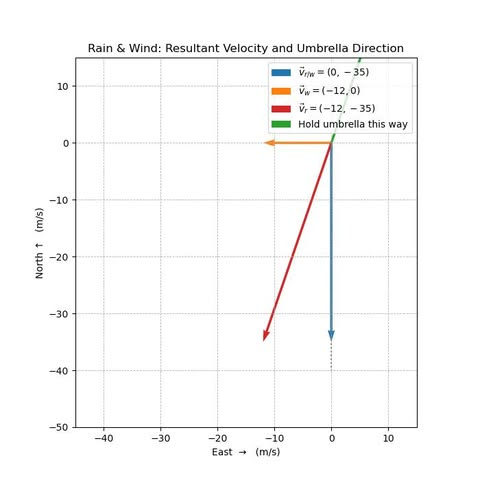
\includegraphics[scale=0.5]{figs/1.2.24.jpg}
    \caption{}
    \label{fig:1}
\end{figure}
\end{frame}
\end{document}